\Variant{25.05.2025 (1-smena)}
\QQ{1}{$42^n$, $n\in\mathbb N$ ning qanday eng kiçik qiymatida $49^5\cdot12^3$ soniga qoldiqsiz bölinadi?
\Opts{$5$}{$8$}{$9$}{$10$}}
\QQ{2}{Hisoblang:
\[\sqrt{\frac{2026!}{2025!+2024!}}-\sqrt{\frac{10!}{9!+8!}}\]
\Opts{$43$}{$42$}{$44$}{$45$}}
\QQ{3}{$1$ soatda Anvar $20$ ta detal, Sardor $21$ ta detal işlab çiqardi. Ikkalasi bir xil miqdorda detal yasadi va Sardor işni $10$ daqiqa oldin tugatgan bölsa, har biri neçtadan detal yasagan?
\Opts{$60$}{$70$}{$80$}{$90$}}
\QQ{4}{Zavodda $4020$ ta avtomobil $1$ oyda işlab çiqarildi. Bu bir oylik rejaning $120\%$ ini taşkil etadi. Zavodda rejadan taşqari neçta avtomobil işlab çiqarilgan?
\Opts{$804$}{$700$}{$670$}{$750$}}
\QQ{5}{Hisoblang:
\[\frac{2^{98}+1}{2^{49}+2^{25}+1}\]
\Opts{$2^{50}-2^{24}+1$}{$2^{49}-2^{25}+1$}{$2^{49}+2^{25}+1$}{$2^{50}+2^{24}+1$}}
\QQ{6}{Sonlarni kamayiş tartibida yozing:
\[a=\sqrt[6]{26},\quad b=\sqrt[3]5,\quad c=\sqrt3\]
\Opts{$c>b>a$}{$a>b>c$}{$c>a>b$}{$a>c>b$}}
\QQ{7}{Agar $2025^3-2023^3=a$ bölsa, $\sqrt{\dfrac{a-2}6}$ ni toping.
\Opts{$2021$}{$2025$}{$2023$}{$2024$}}
\QQ{8}{Agar arifmetik progressiyada $a_1+a_m=90$ va $S_m=270$ ga teng bölsa, $m$ ni toping.
\Opts{$5$}{$6$}{$8$}{$9$}}
\QQ{9}{Arifmetik va geometrik progressiya uçun $a_1=b_1=1$, $a_9=b_9$ va $a_1+a_2+\dots+a_9=369$ bölsa, $b_7$ ni toping.
\Opts{$27$}{$54$}{$36$}{$48$}}
\QQ{10}{Agar $\left(\dfrac1{625}\right)^{a^2+4ab}=\left(\sqrt[3]{625}\right)^{3a^2-10ab}$ tenglik örinli bölsa ($ab\ne0$), $\dfrac ab$ ni toping.
\Opts{$\dfrac2{21}$}{$-\dfrac13$}{$\dfrac5{21}$}{$\dfrac8{21}$}}
\QQ{11}{Agar $a+b+c=0$ va $a^2+b^2+c^2=1$ bölsa, $a^4+b^4+c^4$ ni toping.
\Opts{$\dfrac12$}{$\dfrac14$}{$\dfrac18$}{$\dfrac23$}}
\QQ{12}{Hisoblang:
\[\arcsin\left(-\frac{\sqrt3}2\right)+\arctg\left(\frac{\sqrt3}3\right)\]
\Opts{$-\dfrac\pi6$}{$\dfrac\pi6$}{$\dfrac\pi3$}{$-\dfrac\pi3$}}
\QQ{13}{Agar $\sin\alpha-\cos\alpha=\dfrac1{\sqrt5}$, $\alpha\in\left(0;\,\dfrac\pi2\right)$ bölsa, $\sin2\alpha-\cos2\alpha$ ni toping.
\Opts{$\dfrac15$}{$\dfrac35$}{$\dfrac65$}{$\dfrac75$}}
\QQ{14}{Tenglama neçta yeçimga ega?
\[222^{3x}+222^x=222\]
\Opts{Haqiqiy yeçimi yöq}{$1$}{$2$}{$3$}}
\QQ{15}{Tenglama neçta haqiqiy ildizga ega?
\[\left(\frac14\right)^{\frac{\log_{12}\log_8x}{\log_{12}0{,}25}}=\log_{\frac18}3\]
\Opts{Çeksiz köp}{Haqiqiy ildizga ega emas}{$1$}{$2$}}
\QQ{16}{$|x-4|-\sqrt{4x+17}=-3$ tenglamaning haqiqiy ildizlari yiğindisini toping.
\Opts{$10$}{$8$}{$26$}{$2$}}
\QQ{17}{Tenglamaning haqiqiy ildizlari yiğindisini toping (agar u bitta bölsa öşa ildizni toping).
\[x\sqrt x-4x+3\sqrt x=4x-16\sqrt x+12\]
\Opts{$25$}{$26$}{$17$}{$10$}}
\QQ{18}{$[-20;\,20]$ kesmada tengsizlik neçta butun yeçimga ega?
\[\sqrt{x^2-10x+16}<2x-4\]
\Opts{$10$}{$11$}{$12$}{$13$}}
\QQ{19}{$\sqrt{x^2+9}<5$ neçta natural son tengsizlikni qanoatlantiradi?
\Opts{$3$}{$4$}{$5$}{$6$}}
\QQ{20}{Agar $g(x)=6x-5$, $g(f(x))=x^2$ ga teng bölsa, $f(2)$ ni toping.
\Opts{$1$}{$\dfrac32$}{$2$}{$\dfrac52$}}
\QQ{21}{Aniq integralni hisoblang:
\[\int_{\frac\pi2}^{\frac{2\pi}3}\frac1{1+\sin x+\cos x}\,dx\]
\Opts{$\ln\dfrac{\sqrt3+1}2$}{$\ln\dfrac{\sqrt3-1}2$}{$\ln\dfrac{\sqrt3+2}2$}{$\ln\dfrac{\sqrt3-2}2$}}
\QQ{22}{Agar $g(x)=\dfrac{x+1}x$ va $g(f(x))=\dfrac{x-1}{x-2}$ bölsa, $f(2023)$ ni toping.
\Opts{$2$}{$2021$}{$2023$}{$2025$}}
\QQ{23}{$f(x)=\dfrac{\cos^2x+6\cos x+9}{\sin^2x}$ funksiyaning $\left[-\dfrac\pi3;\,\dfrac{3\pi}2\right]$ oraliqdagi eng kiçik qiymatini toping.
\Opts{$5$}{$9$}{$8$}{$10$}}
\QQ{24}{Rasmda aylana va töğri törtburçak tasvirlangan. Aylana bilan çegaralangan soha yuzining töğri törtburçak yuziga nisbatini toping.
\qfig{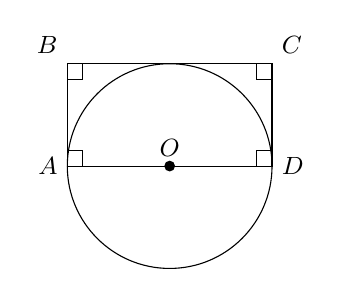
\begin{tikzpicture}[scale=1.3,font=\small]
\coordinate (A) at (-1,0); \coordinate (D) at (1,0); \coordinate (C) at (1,1); \coordinate (B) at (-1,1); \coordinate (O) at (0,0);
\draw (O) circle (1); \draw (A)--(B)--(C)--(D)--cycle; \fill (O) circle (1.5pt);
\draw (-1,0.15)--(-0.85,0.15)--(-0.85,0); \draw (-1,0.85)--(-0.85,0.85)--(-0.85,1); \draw (1,0.85)--(0.85,0.85)--(0.85,1); \draw (1,0.15)--(0.85,0.15)--(0.85,0);
\node[left] at (A) {$A$}; \node[above left] at (B) {$B$}; \node[above right] at (C) {$C$}; \node[right] at (D) {$D$}; \node[above] at (O) {$O$};
\end{tikzpicture}}
\Opts{$\dfrac\pi2$}{$\dfrac{3\pi}4$}{$\dfrac\pi4$}{$\pi$}}
\QQ{25}{$ABC$ uçburçakka içki çizilgan aylananing markazi $O$ nuqta. Agar $BC=8$, $AB=13$ va $\angle AOB=150^\circ$ bölsa, $ABC$ uçburçak yuzini toping.
\qfig{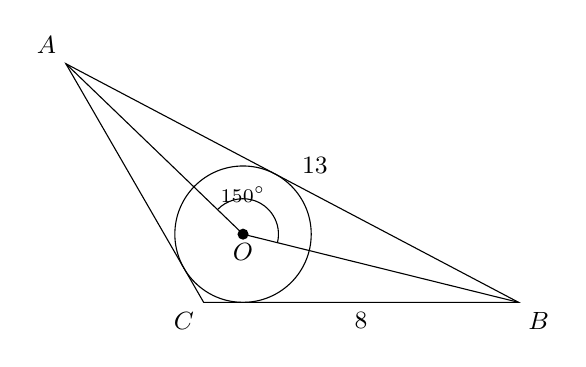
\begin{tikzpicture}[scale=0.5,font=\small]
\coordinate (C) at (0,0); \coordinate (B) at (8,0); \coordinate (A) at (-3.5,6.062); \coordinate (O) at (1,1.732);
\draw (A)--(B)--(C)--cycle; \draw (O) circle (1.732); \draw (A)--(O)--(B); \fill (O) circle (4pt);
\draw (O)+(-13.9:0.9) arc (-13.9:136.1:0.9);
\node[below left] at (C) {$C$}; \node[below right] at (B) {$B$}; \node[above left] at (A) {$A$}; \node[below] at (O) {$O$};
\node[below] at (4,0) {$8$}; \node[above right] at (2.25,3.03) {$13$}; \node[above] at (1,2.3) {\scriptsize$150^\circ$};
\end{tikzpicture}}
\Opts{$28$}{$12\sqrt3$}{$14\sqrt3$}{$24$}}
\QQ{26}{$ABCD$ parallelogrammning $A$ va $B$ burçak bissektrisalari $F$ nuqtada kesişadi. Agar parallelogramm yuzi $48$ ga teng bölsa, $AFD$ uçburçak yuzini toping.
\qfig{\begin{tikzpicture}[scale=0.75,font=\small]
\coordinate (A) at (0,0); \coordinate (D) at (6,0); \coordinate (B) at (1.5,2.6); \coordinate (C) at (7.5,2.6); \coordinate (F) at (2.25,1.3);
\fill[qfill] (A)--(F)--(D)--cycle;
\draw (A)--(B)--(C)--(D)--cycle; \draw (A)--(F)--(D); \draw (B)--(F);
\draw (A)+(0:0.5) arc (0:30:0.5); \draw (A)+(30:0.6) arc (30:60:0.6);
\node[below left] at (A) {$A$}; \node[below right] at (D) {$D$}; \node[above left] at (B) {$B$}; \node[above right] at (C) {$C$}; \node[below] at (F) {$F$};
\end{tikzpicture}}
\Opts{$21$}{$18$}{$15$}{$12$}}
\QQ{27}{Muntazam $ABC$ uçburçak içidan $F$ nuqta olingan. Bunda $F$ nuqtadan $AC$ va $BC$ tomonlargaça bölgan eng qisqa masofalar teng, $F$ nuqtadan $AB$ tomongaça bölgan eng qisqa masofa $1$ ga teng. Agar $AB=4\sqrt3$ ga teng bölsa, $F$ nuqtadan $AC$ tomongaça bölgan eng qisqa masofani toping.
\Opts{$5$}{$2{,}5$}{$3$}{$3{,}5$}}
\QQ{28}{Rasmda $ABCDEFKM$ muntazam sakkizburçak tasvirlangan, $L=MC\cap BF$. $\dfrac{S_2}{S_1}$ nisbatini toping.
\qfig{\begin{tikzpicture}[scale=1.25,font=\small]
\coordinate (A) at (-0.5,1.207); \coordinate (B) at (0.5,1.207); \coordinate (C) at (1.207,0.5); \coordinate (D) at (1.207,-0.5); \coordinate (E) at (0.5,-1.207); \coordinate (F) at (-0.5,-1.207); \coordinate (K) at (-1.207,-0.5); \coordinate (M) at (-1.207,0.5); \coordinate (L) at (0.207,0.5);
\fill[qfill] (L)--(B)--(C)--cycle; \fill[qfill] (M)--(L)--(F)--(K)--cycle;
\draw (A)--(B)--(C)--(D)--(E)--(F)--(K)--(M)--cycle; \draw (M)--(C); \draw (B)--(F);
\node[above left] at (A) {$A$}; \node[above right] at (B) {$B$}; \node[right] at (C) {$C$}; \node[right] at (D) {$D$}; \node[below right] at (E) {$E$}; \node[below left] at (F) {$F$}; \node[left] at (K) {$K$}; \node[left] at (M) {$M$}; \node[above left] at (L) {$L$};
\node at (0.62,0.75) {$S_1$}; \node at (-0.8,0) {$S_2$};
\end{tikzpicture}}
\Opts{$\sqrt2+1$}{$\sqrt2+2$}{$\sqrt2+3$}{$\sqrt2+4$}}
\QQ{29}{Rasmda muntazam $ABCDEF$ oltiburçak tasvirlangan: $A$ va $F$ uçlari $Ox$ öqida, $B$ uçi $Oy$ öqida, $D(x;\,6)$. $E$ nuqtaning koordinatalari köpaytmasini toping.
\qfig{\begin{tikzpicture}[scale=0.42,font=\small]
\draw[-{Stealth[length=4pt]}] (-1.5,0)--(8.5,0) node[right] {$x$}; \draw[-{Stealth[length=4pt]}] (0,-1)--(0,7.3) node[left] {$y$};
\coordinate (A) at (1.732,0); \coordinate (F) at (5.196,0); \coordinate (E) at (6.928,3); \coordinate (D) at (5.196,6); \coordinate (C) at (1.732,6); \coordinate (B) at (0,3);
\draw (A)--(B)--(C)--(D)--(E)--(F)--cycle;
\node[below] at (A) {$A$}; \node[below] at (F) {$F$}; \node[right] at (E) {$E$}; \node[above right] at (D) {$D(x;\,6)$}; \node[above left] at (C) {$C$}; \node[left] at (B) {$B$}; \node[below left] at (0,0) {$O$};
\end{tikzpicture}}
\Opts{$8$}{$9$}{$9\sqrt3$}{$12\sqrt3$}}
\QQ{30}{Uçburçakning tomonlari $10$, $17$ va $21$ ga teng. Uçburçakning katta burçagi uçidan tekislikka perpendikulyar ötkazilgan (uzunligi $15$). Bu perpendikulyarning tekislikdan taşqaridagi uçidan uçburçakning katta tomonigaça bölgan masofani aniqlang.
\Opts{$17$}{$16$}{$18$}{$20$}}
\QQ{31}{Rasmda Venn diagrammasi berilgan. $(A\cup B)\cap C$ ning qism töplamlar sonini toping.
\qfig{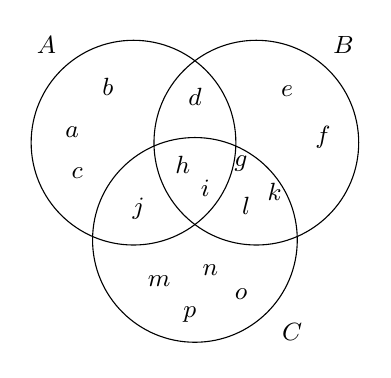
\begin{tikzpicture}[scale=1.3,font=\small]
\draw (-0.6,0.5) circle (1); \draw (0.6,0.5) circle (1); \draw (0,-0.45) circle (1);
\node at (-1.45,1.45) {$A$}; \node at (1.45,1.45) {$B$}; \node at (0.95,-1.35) {$C$};
\node at (-1.2,0.6) {$a$}; \node at (-0.85,1.05) {$b$}; \node at (-1.15,0.2) {$c$}; \node at (0,0.95) {$d$}; \node at (0.9,1.0) {$e$}; \node at (1.25,0.55) {$f$};
\node at (-0.12,0.28) {$h$}; \node at (0.1,0.05) {$i$}; \node at (-0.55,-0.15) {$j$}; \node at (0.45,0.3) {$g$}; \node at (0.5,-0.12) {$l$}; \node at (0.78,0.02) {$k$};
\node at (-0.35,-0.85) {$m$}; \node at (0.15,-0.75) {$n$}; \node at (0.45,-0.98) {$o$}; \node at (-0.05,-1.18) {$p$};
\end{tikzpicture}}
\Opts{$32$}{$64$}{$128$}{$256$}}
\QQ{32}{Seyf maxfiy $6$ xonali kod bilan oçiladi. Kodlar raqamlardan iborat. Eng köpi bilan seyfni neça xil usulda oçiş mumkin?
\Opts{$10^5$}{$9\cdot10^5$}{$10!$}{$10^6$}}
\QQ{33}{\Moslash{Rasmda qirralari $2$ ga teng bölgan $ABCDEFA_1B_1C_1D_1E_1F_1$ muntazam oltiburçakli prizma tasvirlangan.
\par\centering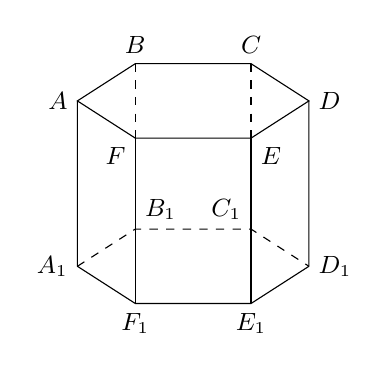
\begin{tikzpicture}[scale=1.05,font=\small]
\coordinate (A) at (-1.4,2); \coordinate (B) at (-0.7,2.45); \coordinate (C) at (0.7,2.45); \coordinate (D) at (1.4,2); \coordinate (E) at (0.7,1.55); \coordinate (F) at (-0.7,1.55);
\coordinate (A1) at (-1.4,0); \coordinate (B1) at (-0.7,0.45); \coordinate (C1) at (0.7,0.45); \coordinate (D1) at (1.4,0); \coordinate (E1) at (0.7,-0.45); \coordinate (F1) at (-0.7,-0.45);
\draw (A)--(B)--(C)--(D)--(E)--(F)--cycle; \draw (A)--(A1)--(F1)--(E1)--(D1)--(D); \draw (F)--(F1); \draw (E)--(E1);
\draw[dashed] (A1)--(B1)--(C1)--(D1); \draw[dashed] (B)--(B1); \draw[dashed] (C)--(C1);
\node[left] at (A) {$A$}; \node[above] at (B) {$B$}; \node[above] at (C) {$C$}; \node[right] at (D) {$D$}; \node[below right] at (E) {$E$}; \node[below left] at (F) {$F$};
\node[left] at (A1) {$A_1$}; \node[above right] at (B1) {$B_1$}; \node[above left] at (C1) {$C_1$}; \node[right] at (D1) {$D_1$}; \node[below] at (E1) {$E_1$}; \node[below] at (F1) {$F_1$};
\end{tikzpicture}}{A) $12$\par B) $4\sqrt6$\par C) $8$\par D) $3\sqrt6$\par E) $3\sqrt7$\par F) $4\sqrt7$}{$ACD_1F_1$ törtburçak yuzini toping.}{$BC_1D_1E$ törtburçak yuzini toping.}{$A$, $B$, $E_1$ nuqtalardan ötuvçi kesim yuzini toping.}}
\QQ{36}{Tenglamalar sistemasi:
\[\begin{cases}x^2+y^2=36,\\ |x|+y=a\end{cases}\]
\AB{Sistemaning $3$ ta yeçimga ega böladigan $a$ larning yiğindisini toping.}{Sistemaning $4$ ta yeçimga ega böladigan $a$ ning butun qiymatlari yiğindisini toping.}}
\QQ{37}{Tenglamani yeçing:
\[\frac{0{,}5-\cos2x}{\cos2x-\sin x-1}=\cos2x+\sin x-1\]
\AB{Tenglamaning eng kiçik musbat va eng katta manfiy yeçimlari yiğindisini toping.}{Tenglama $[-\pi;\,\pi]$ oraliğida neçta yeçimga ega?}}
\QQ{38}{Rasmda $f(x)=ax^2+bx+c$ va $g(x)=k\sqrt{x+1}+l$ funksiyalar grafiklari berilgan. $f(x)$ grafigi $Ox$ ni $(m;\,0)$ va $(5;\,0)$ nuqtalarda kesib ötadi, uçi $(2;\,-4{,}5)$ da. $f(x)$ va $g(x)$ grafiklari $(0;\,n)$ va $(m;\,0)$ nuqtalarda kesişadi.
\qfig{\begin{tikzpicture}[x=0.5cm,y=0.42cm,font=\small]
\draw[-{Stealth[length=4pt]}] (-3,0)--(7,0) node[right] {$x$}; \draw[-{Stealth[length=4pt]}] (0,-7)--(0,4) node[left] {$y$};
\draw[thick,domain=-1.9:5.85,samples=60] plot (\x,{0.5*\x*\x-2*\x-2.5}); \draw[thick,domain=-1:6.2,samples=80] plot (\x,{-2.5*sqrt(\x+1)});
\fill (-1,0) circle (2.5pt); \fill (5,0) circle (2.5pt); \fill (0,-2.5) circle (2.5pt); \fill (2,-4.5) circle (2.5pt);
\node[above left] at (-1,0) {$(m;0)$}; \node[above] at (5,0) {$(5;0)$}; \node[left] at (0,-2.5) {$(0;n)$}; \node[below] at (2,-4.7) {$(2;-4{,}5)$};
\node[right] at (5.7,3) {$f(x)$}; \node[right] at (6.2,-6.6) {$g(x)$};
\end{tikzpicture}}
\AB{$f(-2)$ ni toping.}{$\dfrac{a-b-l-c}{k-m-n}$ ni toping.}}
\QQ{39}{Agar $f(0)=1$, $f'(0)=2$ va $f''(x)=4f'(x)-3f(x)+1$ bölsa:
\AB{$f''(0)$ ni toping.}{$f^{(4)}(0)$ ni toping.}}
\QQ{40}{Rasmda $y=k_1x+l_1$, $y=k_2x+l_2$ töğri çiziqlar va $y=ax^2+bx+c$ parabola tasvirlangan. $y=k_2x+l_2$ töğri çiziq $(0;\,6)$ va $(12;\,0)$ nuqtalardan ötadi; $y=k_1x+l_1$ töğri çiziq unga $(0;\,6)$ nuqtada perpendikulyar va parabolaga şu nuqtada urinadi. Parabola $(6;\,0)$ nuqtadan ötadi, $B$ — parabola va $y=k_2x+l_2$ ning ikkinçi kesişiş nuqtasi.
\qfig{\begin{tikzpicture}[scale=0.38,font=\small]
\draw[-{Stealth[length=4pt]}] (-4,0)--(14,0) node[right] {$x$}; \draw[-{Stealth[length=4pt]}] (0,-2)--(0,11) node[left] {$y$};
\fill[qfill] (0,0)--(5,3.5)--(6,0)--cycle; \draw (5,3.5)--(6,0);
\draw[thick,domain=-1.6:6.3,samples=60] plot (\x,{-0.5*\x*\x+2*\x+6});
\draw (-3.5,-1)--(2.2,10.4); \draw (-3,7.5)--(13.5,-0.75); \draw (0,0)--(5,3.5);
\draw (0,6)++(-0.45,0.225)--++(0.2,0.4)--++(0.45,-0.225);
\fill (0,6) circle (4pt); \fill (5,3.5) circle (4pt); \fill (6,0) circle (4pt); \fill (12,0) circle (4pt);
\node[above right] at (0,6) {$(0;6)$}; \node[above right] at (5,3.5) {$B$}; \node[below right] at (6,0) {$(6;0)$}; \node[below] at (12,0) {$(12;0)$}; \node[below left] at (0,0) {$O$};
\node[right] at (2.2,10.4) {$y=k_1x+l_1$}; \node[above] at (-3.4,7.6) {$y=k_2x+l_2$}; \node[right] at (4.2,8.6) {$y=ax^2+bx+c$};
\end{tikzpicture}}
\AB{$B$ nuqta koordinatalari yiğindisini toping.}{Böyalgan uçburçak yuzini toping.}}
\QQ{41}{Markazi $O$ bölgan muntazam $ABC$ uçburçak içidagi $P$ nuqta uçun $OC=\dfrac{14\sqrt3}3$, $PB=10$, $AP=6$.
\qfig{\begin{tikzpicture}[scale=0.32,font=\small]
\coordinate (A) at (0,0); \coordinate (C) at (14,0); \coordinate (B) at (7,12.124); \coordinate (O) at (7,4.041); \coordinate (P) at (5.571,2.227);
\fill[qfill] (A)--(B)--(P)--cycle;
\draw (A)--(B)--(C)--cycle; \draw (O) circle (4.041); \draw (A)--(P)--(B); \draw (P)--(C); \draw (O)--(C); \fill (O) circle (5pt);
\node[below left] at (A) {$A$}; \node[above] at (B) {$B$}; \node[below right] at (C) {$C$}; \node[above] at (O) {$O$}; \node[below] at (P) {$P$};
\end{tikzpicture}}
\AB{Böyalgan soha ($ABP$ uçburçak) yuzini toping.}{$PC$ ni toping.}}
\QQ{42}{Tomonlari $13$, $13$, $15$, $15$ bölgan qavariq törtburçakka aylana içki çizilgan. Diagonallardan biri kesişiş nuqtasida $5:9$ nisbatda bölinadi.
\AB{Törtburçakning yuzini toping.}{Diagonallar kesişiş nuqtasidan aylana markazigaça bölgan masofani toping.}}
\QQ{43}{Muntazam $ABCDEF$ oltiburçakda $P$ — $AE$ va $FC$ diagonallarning kesişiş nuqtasi.
\qfig{\begin{tikzpicture}[scale=0.4,font=\small]
\coordinate (F) at (-4,0); \coordinate (C) at (4,0); \coordinate (E) at (-2,3.464); \coordinate (D) at (2,3.464); \coordinate (A) at (-2,-3.464); \coordinate (B) at (2,-3.464); \coordinate (P) at (-2,0);
\fill[qfill] (E)--(P)--(F)--cycle; \fill[qfill] (P)--(D)--(C)--cycle;
\draw (A)--(B)--(C)--(D)--(E)--(F)--cycle; \draw (F)--(C); \draw (E)--(A); \draw (P)--(D);
\node[left] at (F) {$F$}; \node[right] at (C) {$C$}; \node[above left] at (E) {$E$}; \node[above right] at (D) {$D$}; \node[below left] at (A) {$A$}; \node[below right] at (B) {$B$}; \node[below right] at (P) {$P$};
\end{tikzpicture}}
\AB{Tomoni $4$ ga teng bölsa, $PDC$ uçburçak yuzini toping.}{$EPF$ uçburçak yuzining $ABCP$ törtburçak yuziga nisbatini toping.}}
\QQ{44}{Muntazam oltiburçakli kesik piramidaning içida kub joylaşgan: kubning pastki yoği katta asosda, yuqori yoğining uçlari kiçik asos tomonlarida yotadi. Kesik piramidaning kiçik asosi yuzi katta asosidan $4$ marta kiçik.
\qfig{\begin{tikzpicture}[scale=0.9,font=\small]
\coordinate (P1) at (-2.4,0); \coordinate (P2) at (-1.2,-0.55); \coordinate (P3) at (1.2,-0.55); \coordinate (P4) at (2.4,0); \coordinate (P5) at (1.2,0.55); \coordinate (P6) at (-1.2,0.55);
\coordinate (Q1) at (-1.2,1.6); \coordinate (Q2) at (-0.6,1.325); \coordinate (Q3) at (0.6,1.325); \coordinate (Q4) at (1.2,1.6); \coordinate (Q5) at (0.6,1.875); \coordinate (Q6) at (-0.6,1.875);
\draw (P1)--(P2)--(P3)--(P4); \draw[dashed] (P4)--(P5)--(P6)--(P1);
\draw (Q1)--(Q2)--(Q3)--(Q4)--(Q5)--(Q6)--cycle; \draw (P1)--(Q1); \draw (P2)--(Q2); \draw (P3)--(Q3); \draw (P4)--(Q4); \draw[dashed] (P5)--(Q5); \draw[dashed] (P6)--(Q6);
\fill[qfill] (-0.76,0.14)--(0.4,0.14)--(0.4,1.42)--(-0.76,1.42)--cycle;
\draw[black!75] (-0.76,0.14)--(0.4,0.14)--(0.4,1.42)--(-0.76,1.42)--cycle;
\draw[black!75] (-0.76,1.42)--(-0.4,1.78)--(0.76,1.78)--(0.4,1.42); \draw[black!75] (0.76,1.78)--(0.76,0.5)--(0.4,0.14);
\draw[black!75,dashed] (-0.76,0.14)--(-0.4,0.5)--(0.76,0.5); \draw[black!75,dashed] (-0.4,0.5)--(-0.4,1.78);
\end{tikzpicture}}
\AB{Kiçik asos tomoni $1+\sqrt3$ ga teng bölsa, kub hajmini toping.}{Kubning töla sirti $24-12\sqrt3$ ga teng bölsa, katta asos tomonini toping.}}
\QQ{45}{$A$ şahar va $C$ qişloq kengligi $DE=20$ km bölgan daryoning (qirğoqlari parallel) turli tomonlarida joylaşgan. $A$ dan qirğoqqaça masofa $AB=30$ km, $C$ dan ikkinçi qirğoqqaça masofa $FC=50$ km, $AC=20\sqrt{34}$ km. Daryoga qirğoqlarga perpendikulyar $DE$ köprik şunday qurilişi kerakki, $A$ dan $C$ gaça $AD+DE+EC$ yöl eng qisqa bölsin.
\qfig{\begin{tikzpicture}[scale=0.42,font=\small]
\fill[qfill] (-2,-2) rectangle (9,0);
\coordinate (A) at (0,3); \coordinate (B) at (0,0); \coordinate (D) at (2.25,0); \coordinate (E) at (2.25,-2); \coordinate (F) at (6,-2); \coordinate (C) at (6,-7);
\draw[{Stealth[length=4pt]}-{Stealth[length=4pt]}] (A)--(B); \draw[{Stealth[length=4pt]}-{Stealth[length=4pt]}] (F)--(C); \draw[thick] (D)--(E);
\draw (B)--(D); \draw (E)--(F); \draw[dashed] (A)--(D); \draw[dashed] (E)--(C);
\fill (A) circle (3pt); \fill (C) circle (3pt);
\node[left] at (A) {$A$}; \node[left] at (B) {$B$}; \node[above right] at (D) {$D$}; \node[below left] at (E) {$E$}; \node[above right] at (F) {$F$}; \node[right] at (C) {$C$};
\node[left] at (0,1.5) {$30$}; \node[right] at (6,-4.5) {$50$}; \node[right] at (2.25,-1) {$20$};
\end{tikzpicture}}
\AB{$BD$ ni toping.}{$AD+DE+EC$ ning eng kiçik qiymatini toping.}}
\Javoblar{D B B C B C D B A B A A D B B A B D A B A B C A C D B C D A B D B E A}{%
\OK{36}{$6$}{$15$}\OK{37}{$-\dfrac\pi{12}$}{$6$}\OK{38}{$3{,}5$}{$5$}\OK{39}{$6$}{$54$}\OK{40}{$8{,}5$}{$10{,}5$}%
\OK{41}{$15\sqrt3$}{$2\sqrt{19}$}\OK{42}{$168$}{$1{,}5$}\OK{43}{$6\sqrt3$}{$\dfrac15$}\OK{44}{$24\sqrt3$}{$\dfrac{2\sqrt3}3$}\OK{45}{$22{,}5$}{$120$}}
